\documentclass[week7]{csse2002}
\usepackage{slides}

\author{Brae Webb}

\title{CSSE2002 Week 7 Tutorial}
 
\begin{document}

\begin{frame}
\maketitle
\end{frame}

\begin{topic}{Admin}
\begin{enumerate}
    \item Assignment - you did it!! 🎉
    \item Relax or catchup
\end{enumerate}
\end{topic}

% \begin{topic}{Last Week}
% \begin{java}
% /**
% * Returns true if and only if numbers is an array of ascending
% * integers.
% *
% * @require numbers != null
% * @ensure \result is true iff for all indices j such that
% * 0 <= j < a.length - 1, a[j] <= a[j + 1]
% */
% public boolean ascending(int[] numbers) {
% 	boolean result = true;
% 	for (int i = 0; i < numbers.length - 1; i++) {
% 		if (numbers[i] > numbers[i + 1]) {
% 			result = false;
% 		}
% 	}
% 	return result;
% }
% \end{java}
% \end{topic}

\begin{topic}{This Week...}
\begin{enumerate}
    \item instanceof
    \item Method resolution
\end{enumerate}
\end{topic}

\begin{topic}{instanceof}
\begin{java}
a instanceof A == true
b instanceof A == true

x instanceof Y
\end{java}

Simply, is x a direct instance of class Y or an instance of a subclass of Y.
\end{topic}

\begin{topic}{Method Resolution}
\begin{subtopic}{1}
\textbf{White lie: } Method resolution only cares about the runtime type.

\begin{java}
class Vehicle {
	int travelTime(Location start, Location end);
	int topSpeed();
}
class Car extends Vehicle {
	int topSpeed();
}

Vehicle vehicle = new Car();
vehicle.topSpeed();
\end{java}

Car.topSpeed()
\end{subtopic}

\begin{subtopic}{2}
"When a method is invoked, the number of actual arguments (and any explicit type arguments) and the compile-time types of the arguments are used, at compile time, to determine the signature of the method that will be invoked. If the method that is to be invoked is an instance method, the actual method to be invoked will be determined at run time, using dynamic method lookup." --- Java language specification

\begin{enumerate}
	\item Signature determined by compile-time type
	\item Lookup of signature by runtime type
\end{enumerate}
\end{subtopic}

\begin{subtopic}{3-}
\begin{java}
class Vehicle {
	int travelTime(Location start, Location end);
	int topSpeed(Vehicle v);
}
class Car extends Vehicle {
	int topSpeed(Car c);
}

Car car = new Car();
Vehicle vehicle = new Car();

vehicle.topSpeed(car);

car.topSpeed(car);
\end{java}
\end{subtopic}

\begin{subtopic}{4-6}
\begin{enumerate}
	\item Signature determined by compile-time type
	\item Lookup of signature by runtime type
\end{enumerate}
\end{subtopic}

\begin{subtopic}{5}
\begin{enumerate}
	\item topSpeed(Vehicle)
	\item no topSpeed(Vehicle) in Car, so Vehicle.topSpeed(Vehicle)
\end{enumerate}
\end{subtopic}

\begin{subtopic}{6}
\begin{enumerate}
	\item topSpeed(Car)
	\item topSpeed(Car) in Car, so Car.topSpeed(Car)
\end{enumerate}
\end{subtopic}

\begin{subtopic}{7}
Vehicle.topSpeed(Vehicle)

Car.topSpeed(Car)
\end{subtopic}

\end{topic}


\begin{topic}{Have a good week!}
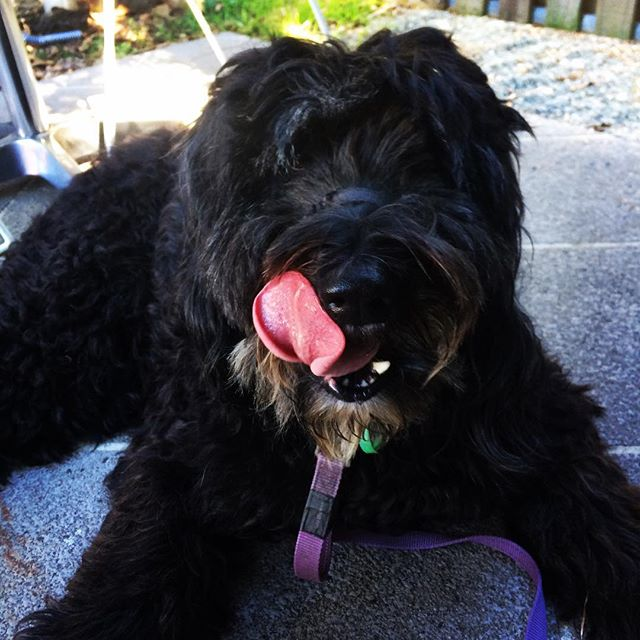
\includegraphics[width=\textwidth,keepaspectratio]{doggo2.jpg}
\end{topic}

\end{document} 
